\documentclass[aspectratio=169]{beamer}

% ---------------------------------------------------------------------------
% Tema e Cores
% ---------------------------------------------------------------------------
\usetheme{Madrid}
\usecolortheme{default}
\setbeamertemplate{navigation symbols}{}
\setbeamertemplate{caption}[numbered]

% ---------------------------------------------------------------------------
% Pacotes
% ---------------------------------------------------------------------------
\usepackage[utf8]{inputenc}
\usepackage[T1]{fontenc}
\usepackage[brazil]{babel}
\usepackage{graphicx}
\usepackage{amsmath}
\usepackage{amssymb}
\usepackage{booktabs}
\usepackage{subcaption}
\usepackage{lmodern}
\usepackage{array}

% ---------------------------------------------------------------------------
% Cores personalizadas (UFCG)
% ---------------------------------------------------------------------------
\definecolor{ufcgblue}{RGB}{0,82,150}
\definecolor{ufcgdark}{RGB}{0,50,100}
\setbeamercolor{palette primary}{bg=ufcgblue,fg=white}
\setbeamercolor{palette secondary}{bg=ufcgdark,fg=white}
\setbeamercolor{palette tertiary}{bg=ufcgdark,fg=white}
\setbeamercolor{palette quaternary}{bg=ufcgblue,fg=white}
\setbeamercolor{structure}{fg=ufcgblue}
\setbeamercolor{section in toc}{fg=ufcgdark}
\setbeamercolor{frametitle}{bg=ufcgblue,fg=white}

\graphicspath{{imgs/}}

% ---------------------------------------------------------------------------
% Informações do documento
% ---------------------------------------------------------------------------
\title[Identificação de Covariâncias de Ruído]{Identificação Adaptativa de Covariâncias\\de Ruído em Filtros de Kalman}
\subtitle{Sistemas Inteligentes -- Atividade 02}
\author[Mateus Pincho]{Mateus Pincho de Oliveira}
\institute[UFCG]{Universidade Federal de Campina Grande (UFCG)\\
Centro de Engenharia Elétrica e Informática (CEEI)}
\date{Abril de 2026}

% ---------------------------------------------------------------------------
\begin{document}

% ---------------------------------------------------------------------------
% Slide de título
% ---------------------------------------------------------------------------
\begin{frame}
    \titlepage
\end{frame}

% ===========================================================================
\section{Motivação}
% ===========================================================================

% ---------------------------------------------------------------------------
\begin{frame}{O Filtro de Kalman Precisa de $Q$ e $R$}
    \begin{block}{Sistema Linear em Tempo Discreto}
        \[
            \mathbf{x}(k{+}1) = F\,\mathbf{x}(k) + \Gamma\,\mathbf{v}(k),
            \qquad \mathbf{v}(k) \sim \mathcal{N}(\mathbf{0},\,Q)
        \]
        \[
            \mathbf{z}(k) = H\,\mathbf{x}(k) + \mathbf{w}(k),
            \qquad \mathbf{w}(k) \sim \mathcal{N}(\mathbf{0},\,R)
        \]
    \end{block}
    \vspace{0.3cm}
    \begin{columns}[T]
        \begin{column}{0.48\textwidth}
            \textbf{$Q$ e $R$ determinam:}
            \begin{itemize}
                \item A covariância de predição $P(k{+}1|k)$
                \item A covariância da inovação $S = HPH' + R$
                \item O ganho de Kalman $W = PH'S^{-1}$
            \end{itemize}
        \end{column}
        \begin{column}{0.48\textwidth}
            \begin{alertblock}{O problema prático}
                Em aplicações reais, $Q$ e $R$ \textbf{não são conhecidos
                a priori}. Escolhas erradas degradam o filtro.
            \end{alertblock}
        \end{column}
    \end{columns}
\end{frame}

% ---------------------------------------------------------------------------
\begin{frame}{Por Que $Q$ e $R$ Incorretos São Problemáticos?}
    \begin{columns}[T]
        \begin{column}{0.48\textwidth}
            \begin{block}{$Q$ muito grande}
                O filtro acredita que a dinâmica é muito imprevisível
                \begin{itemize}
                    \item Confia demais nas medições
                    \item Estimativas ruidosas
                \end{itemize}
            \end{block}
            \vspace{0.2cm}
            \begin{block}{$Q$ muito pequeno}
                O filtro é excessivamente confiante na predição
                \begin{itemize}
                    \item Ignora informações úteis das medições
                    \item Estimativas lentas e enviesadas
                \end{itemize}
            \end{block}
        \end{column}
        \begin{column}{0.48\textwidth}
            \begin{alertblock}{Um problema com 50 anos}
                Desde Mehra (1970), pesquisadores buscam estimar
                $Q$ e $R$ \textbf{diretamente dos dados}.

                \vspace{0.3cm}
                Zhang et al. (2020) propõem uma solução iterativa
                baseada em 6 passos, mais precisa que métodos anteriores.
            \end{alertblock}
            \vspace{0.2cm}
            \textbf{Objetivo:} dado $\{\mathbf{z}(1),\ldots,\mathbf{z}(N)\}$,
            identificar $Q$ e $R$.
        \end{column}
    \end{columns}
\end{frame}

% ---------------------------------------------------------------------------
\begin{frame}{A Sequência de Inovações Como Observável-Chave}
    \begin{block}{Inovação (resíduo de predição)}
        \[
            \boldsymbol{\nu}(k) = \mathbf{z}(k) - H\,\hat{\mathbf{x}}(k|k{-}1)
        \]
        Diferença entre a medição recebida e a medição \textbf{predita}.
    \end{block}
    \vspace{0.2cm}
    \begin{columns}[T]
        \begin{column}{0.52\textwidth}
            \textbf{Propriedade fundamental:}\\
            Para um filtro ótimo, $\{\boldsymbol{\nu}(k)\}$ deve ser
            \textbf{ruído branco} (amostras não correlacionadas).
            \[
                \mathbb{E}[\boldsymbol{\nu}(k)\,\boldsymbol{\nu}(k{-}i)'] =
                \begin{cases} S & i=0 \\ 0 & i\geq 1 \end{cases}
            \]
        \end{column}
        \begin{column}{0.44\textwidth}
            \begin{alertblock}{Ideia central}
                As covariâncias de atraso amostral
                $\hat{C}(i)$ são funções de $Q$ e $R$.
                Inverta essa relação para identificar
                $Q$ e $R$ a partir dos dados.
            \end{alertblock}
        \end{column}
    \end{columns}
\end{frame}

% ===========================================================================
\section{Algoritmo de Seis Passos}
% ===========================================================================

% ---------------------------------------------------------------------------
\begin{frame}{Visão Geral: Algoritmo de Seis Passos}
    \begin{columns}[T]
        \begin{column}{0.50\textwidth}
            \begin{enumerate}
                \item \textbf{Passar o filtro de Kalman} com ganho constante
                      $W^{(r)}$; coletar $\{\boldsymbol{\nu}(k)\}$ e resíduos
                      pós-ajuste $\{\boldsymbol{\mu}(k)\}$
                \item \textbf{Calcular autocovariâncias amostrais} $\hat{C}(i)$,
                      $i = 0,1,\ldots,M-1$
                \item \textbf{Atualizar $W$} via descida de gradiente sobre o
                      objetivo de brancura $J$
            \end{enumerate}
        \end{column}
        \begin{column}{0.47\textwidth}
            \begin{enumerate}
                \setcounter{enumi}{3}
                \item \textbf{Estimar $R$} pela fórmula R3 (garante
                      definição positiva)
                \item \textbf{Estimar $Q$ e $P$} via iteração de Lyapunov
                      com restrições estruturais
                \item \textbf{Laço externo:} re-inicializar $W^{(0)}$ com
                      DARE, repetir até convergência ($\leq 20$ iterações)
            \end{enumerate}
        \end{column}
    \end{columns}
    \vspace{0.3cm}
    \begin{block}{Resultado}
        Ao convergir, o algoritmo entrega estimativas $\hat{Q}$, $\hat{R}$,
        $\hat{W}$, $\hat{S}$ e $\bar{P}$ otimizadas pelos dados.
    \end{block}
\end{frame}

% ---------------------------------------------------------------------------
\begin{frame}{Passos 1--2: Filtro de Kalman e Autocovariâncias}
    \textbf{Passo 1 — Filtro com ganho constante $W$:}
    \[
        \hat{\mathbf{x}}(k{+}1|k) = F\,\hat{\mathbf{x}}(k|k), \qquad
        \boldsymbol{\nu}(k{+}1) = \mathbf{z}(k{+}1) - H\,\hat{\mathbf{x}}(k{+}1|k)
    \]
    \[
        \hat{\mathbf{x}}(k{+}1|k{+}1) = \hat{\mathbf{x}}(k{+}1|k) + W\,\boldsymbol{\nu}(k{+}1), \qquad
        \boldsymbol{\mu}(k{+}1) = \mathbf{z}(k{+}1) - H\,\hat{\mathbf{x}}(k{+}1|k{+}1)
    \]

    \vspace{0.3cm}
    \textbf{Passo 2 — Autocovariância amostral (eq. 50):}
    \[
        \hat{C}(i) = \frac{1}{N-M}\sum_{j=1}^{N-M}\boldsymbol{\nu}(j)\,\boldsymbol{\nu}(j{+}i)',
        \qquad i = 0,1,\ldots,M{-}1
    \]

    \begin{alertblock}{Parâmetro $M$ (número de atrasos)}
        $M$ controla o compromisso entre variância e resolução temporal.
        Deve satisfazer $M \geq n_x$; tipicamente $M \in [40, 100]$.
    \end{alertblock}
\end{frame}

% ---------------------------------------------------------------------------
\begin{frame}{Passo 3: Atualização do Ganho $W$ por Descida de Gradiente}
    \textbf{Objetivo de brancura (eq. 52):}
    \[
        J = \frac{1}{2}\,\text{tr}\!\left\{
            \sum_{i=1}^{M-1}
            \bigl[\text{diag}(\hat{C}(0))\bigr]^{-1/2}
            \hat{C}(i)'\,
            \bigl[\text{diag}(\hat{C}(0))\bigr]^{-1}
            \hat{C}(i)\,
            \bigl[\text{diag}(\hat{C}(0))\bigr]^{-1/2}
        \right\}
    \]
    $J = 0$ significa inovações perfeitamente brancas $\Rightarrow$ filtro ótimo.

    \vspace{0.2cm}
    \textbf{Tamanho de passo adaptativo (Bold Driver, eq. 137):}
    \[
        \alpha^{(r)} =
        \begin{cases}
            0{,}5\;\alpha^{(r-1)} & \text{se}\; J^{(r)} > J^{(r-1)}
                                     \quad\text{(passo muito grande)} \\
            \min\!\bigl(1{,}1\;\alpha^{(r-1)},\;\bar{c}\bigr)
                                  & \text{caso contrário}
                                     \quad\text{(passo aumenta 10\%)}
        \end{cases}
    \]

    \begin{block}{Critérios de parada}
        $\delta_W < 10^{-6}$ \;|\; $\|\nabla_W J\| < 10^{-6}$ \;|\;
        $J < 10^{-6}$ \;|\; 5 iterações sem melhora \;|\; $n_L$ iterações máximas
    \end{block}
\end{frame}

% ---------------------------------------------------------------------------
\begin{frame}{Passo 4: Estimação de $R$ (Fórmula R3)}
    \textbf{Resíduo pós-ajuste:}
    $\boldsymbol{\mu}(k) = (I - HW)\,\boldsymbol{\nu}(k)$
    \quad$\Rightarrow$\quad
    covariância amostral: $\hat{G} = \tfrac{1}{N}\sum_k \boldsymbol{\mu}(k)\boldsymbol{\mu}(k)'$

    \vspace{0.3cm}
    \textbf{Fórmula R3 — equação de Riccati contínua (eq. 78):}
    \[
        \hat{G} = R\,S^{-1}\,R \qquad \text{com } S = \hat{C}(0)
    \]

    \begin{columns}[T]
        \begin{column}{0.52\textwidth}
            \textbf{Solução numérica (Apêndice F):}
            \begin{enumerate}
                \item Cholesky: $S^{-1} = \mathscr{L}\mathscr{L}'$
                \item Eigendecomposição: $\mathscr{L}'\hat{G}\mathscr{L} = U\Lambda U'$
                \item Raiz quadrada: $\mathscr{L}'R\mathscr{L} = U\Lambda^{1/2}U'$
                \item Recuperar: $R = (\mathscr{L}')^{-1}U\Lambda^{1/2}U'\mathscr{L}^{-1}$
            \end{enumerate}
        \end{column}
        \begin{column}{0.44\textwidth}
            \begin{alertblock}{Por que R3?}
                Garante $\hat{R}$ \textbf{definida positiva}
                por construção — as outras fórmulas
                podem produzir autovalores negativos
                devido a erros numéricos.
            \end{alertblock}
        \end{column}
    \end{columns}
\end{frame}

% ---------------------------------------------------------------------------
\begin{frame}{Passos 5--6: Estimação de $Q$/$P$ e Laço Externo}
    \textbf{Passo 5 — Iteração dupla (Lyapunov):}

    \smallskip
    \textit{Inicialização:} $\Gamma Q^{(0)}\Gamma' = WSW'$
    (aproximação de processo de Wiener)

    \textit{Laço interno} (fixado $Q^{(t)}$, iterando em $P$):
    \[
        P^{(\ell+1)} = \Bigl[\bigl(FP^{(\ell)}F' + \Gamma Q^{(t)}\Gamma'\bigr)^{-1}
                        + H'R^{-1}H\Bigr]^{-1}
    \]

    \textit{Atualização de $Q$:}
    \[
        D^{(t+1)} = P + WSW' - FPF', \qquad
        Q^{(t+1)} = \Gamma^{\dagger}\,D^{(t+1)}\,(\Gamma')^{\dagger}
    \]

    \vspace{0.1cm}
    \textbf{Passo 6 — Laço externo (aproximação sucessiva):}
    \begin{itemize}
        \item Com $(\hat{Q},\hat{R})$ atualizados, resolver DARE para novo $W^{(0)}$
        \item Repetir Passos 1--5 (até 20 iterações externas)
        \item Guardar a melhor solução $(W^*, J^*)$ ao longo de todas as iterações
    \end{itemize}
\end{frame}

% ===========================================================================
\section{Caso 1: Sistema Cinemático}
% ===========================================================================

% ---------------------------------------------------------------------------
\begin{frame}{Caso 1 — Descrição do Sistema Cinemático}
    \begin{columns}[T]
        \begin{column}{0.50\textwidth}
            \textbf{Modelo de velocidade constante:}
            \[
                F = \begin{bmatrix} 1 & T \\ 0 & 1 \end{bmatrix},\quad
                H = \begin{bmatrix} 1 & 0 \end{bmatrix},\quad
                \Gamma = \begin{bmatrix} T^2/2 \\ T \end{bmatrix}
            \]
            com $T = 0{,}1\,\text{s}$ (período de amostragem).

            \vspace{0.2cm}
            \textbf{Valores verdadeiros:}
            \[
                Q_{\text{true}} = 0{,}0025, \quad R_{\text{true}} = 0{,}01
            \]
        \end{column}
        \begin{column}{0.47\textwidth}
            \begin{block}{Configuração Monte Carlo}
                \begin{itemize}
                    \item $N = 1000$ amostras por realização
                    \item 100 realizações Monte Carlo
                    \item $M \in \{10,\,20,\,30,\,40,\,50,\,100\}$
                    \item Ganho inicial via DARE com $Q_0 = R_0 = 0{,}1$
                \end{itemize}
            \end{block}
            \vspace{0.2cm}
            \textbf{Métricas reportadas:}\\
            média, IC 95\% e RMSE de
            $\hat{R}$, $\hat{Q}$, $\hat{W}$, $\hat{P}$ em cada valor de $M$.
        \end{column}
    \end{columns}
\end{frame}

% ---------------------------------------------------------------------------
\begin{frame}{Caso 1 — O Que o Artigo Afirma}
    \begin{block}{Afirmações teóricas de Zhang et al. (2020)}
        \begin{itemize}
            \item O algoritmo converge para os valores verdadeiros quando $N \to \infty$
            \item Aumentar $M$ melhora a estimação de $Q$ (mais informação de atraso)
            \item Existe um $M$ ótimo que equilibra variância e viés amostral
            \item As estimativas devem ser \textbf{não enviesadas}: a média das
                  realizações converge para o valor verdadeiro
        \end{itemize}
    \end{block}
    \vspace{0.2cm}
    \begin{columns}[T]
        \begin{column}{0.55\textwidth}
            \textbf{Métrica principal — RMSE:}
            \[
                \text{RMSE}(\hat{\theta}) =
                \sqrt{\frac{1}{N_{\text{MC}}}\sum_{i=1}^{N_{\text{MC}}}
                \!\left(\hat{\theta}^{(i)} - \theta_{\text{true}}\right)^2}
            \]
        \end{column}
        \begin{column}{0.42\textwidth}
            \begin{alertblock}{Nosso objetivo}
                Reproduzir e validar esses resultados
                via simulação, comparando com os
                valores da Tabela 3 do artigo.
            \end{alertblock}
        \end{column}
    \end{columns}
\end{frame}

% ---------------------------------------------------------------------------
\begin{frame}{Caso 1 — RMSE em Função do Número de Atrasos $M$}
    \begin{columns}[T]
        \begin{column}{0.60\textwidth}
            \begin{figure}
                \centering
                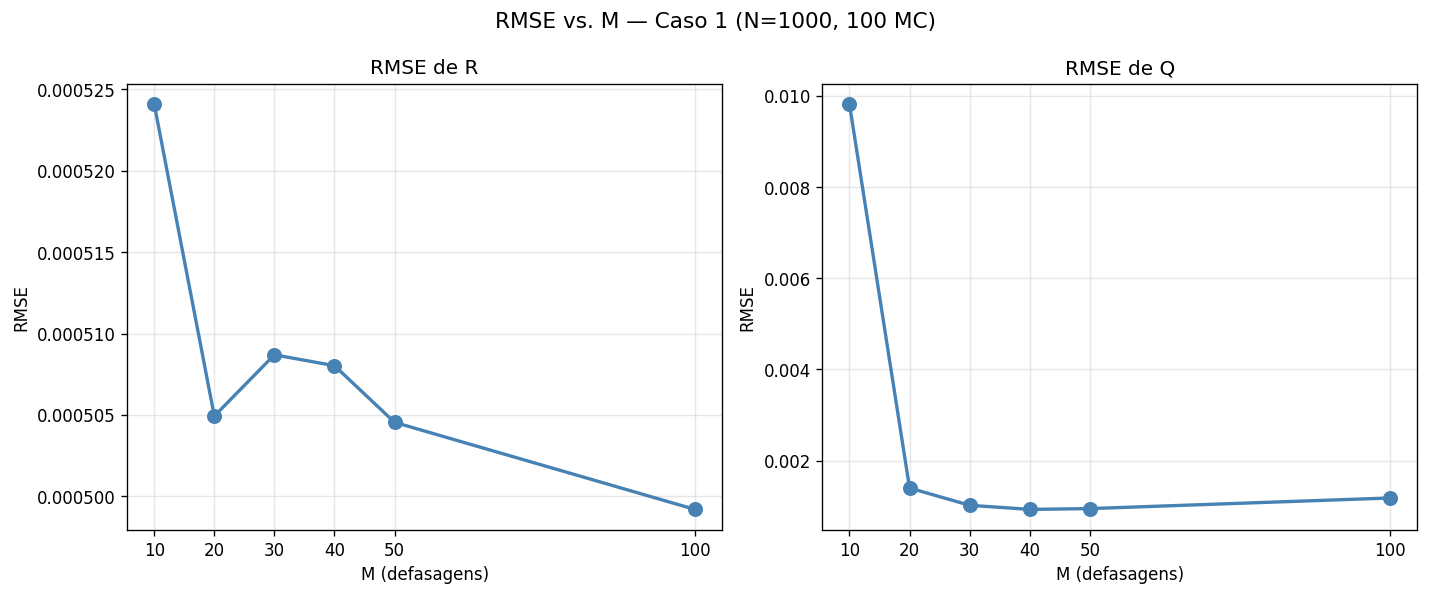
\includegraphics[width=\linewidth]{case1_rmse_vs_M.png}
                \caption{RMSE de $\hat{Q}$ e $\hat{R}$ sobre 100 realizações Monte Carlo,
                         $M \in \{10,20,30,40,50,100\}$.}
            \end{figure}
        \end{column}
        \begin{column}{0.37\textwidth}
            \vspace{0.5cm}
            \begin{block}{Melhor resultado ($M=40$)}
                \begin{tabular}{ll}
                    RMSE($\hat{R}$) & $= 5{,}1\times 10^{-4}$ \\[4pt]
                    RMSE($\hat{Q}$) & $= 9{,}3\times 10^{-4}$
                \end{tabular}
            \end{block}
            \vspace{0.3cm}
            \textbf{Observação:} o RMSE de $\hat{Q}$ decresce com $M$ até
            $M=40$, depois estabiliza (efeito de janelamento).\\[6pt]
            $\hat{R}$ é pouco sensível a $M$ --- estimativa robusta
            ao número de atrasos.
        \end{column}
    \end{columns}
\end{frame}

% ---------------------------------------------------------------------------
\begin{frame}{Caso 1 --- Distribuição Monte Carlo das Estimativas}
    \begin{columns}[T]
        \begin{column}{0.62\textwidth}
            \begin{figure}
                \centering
                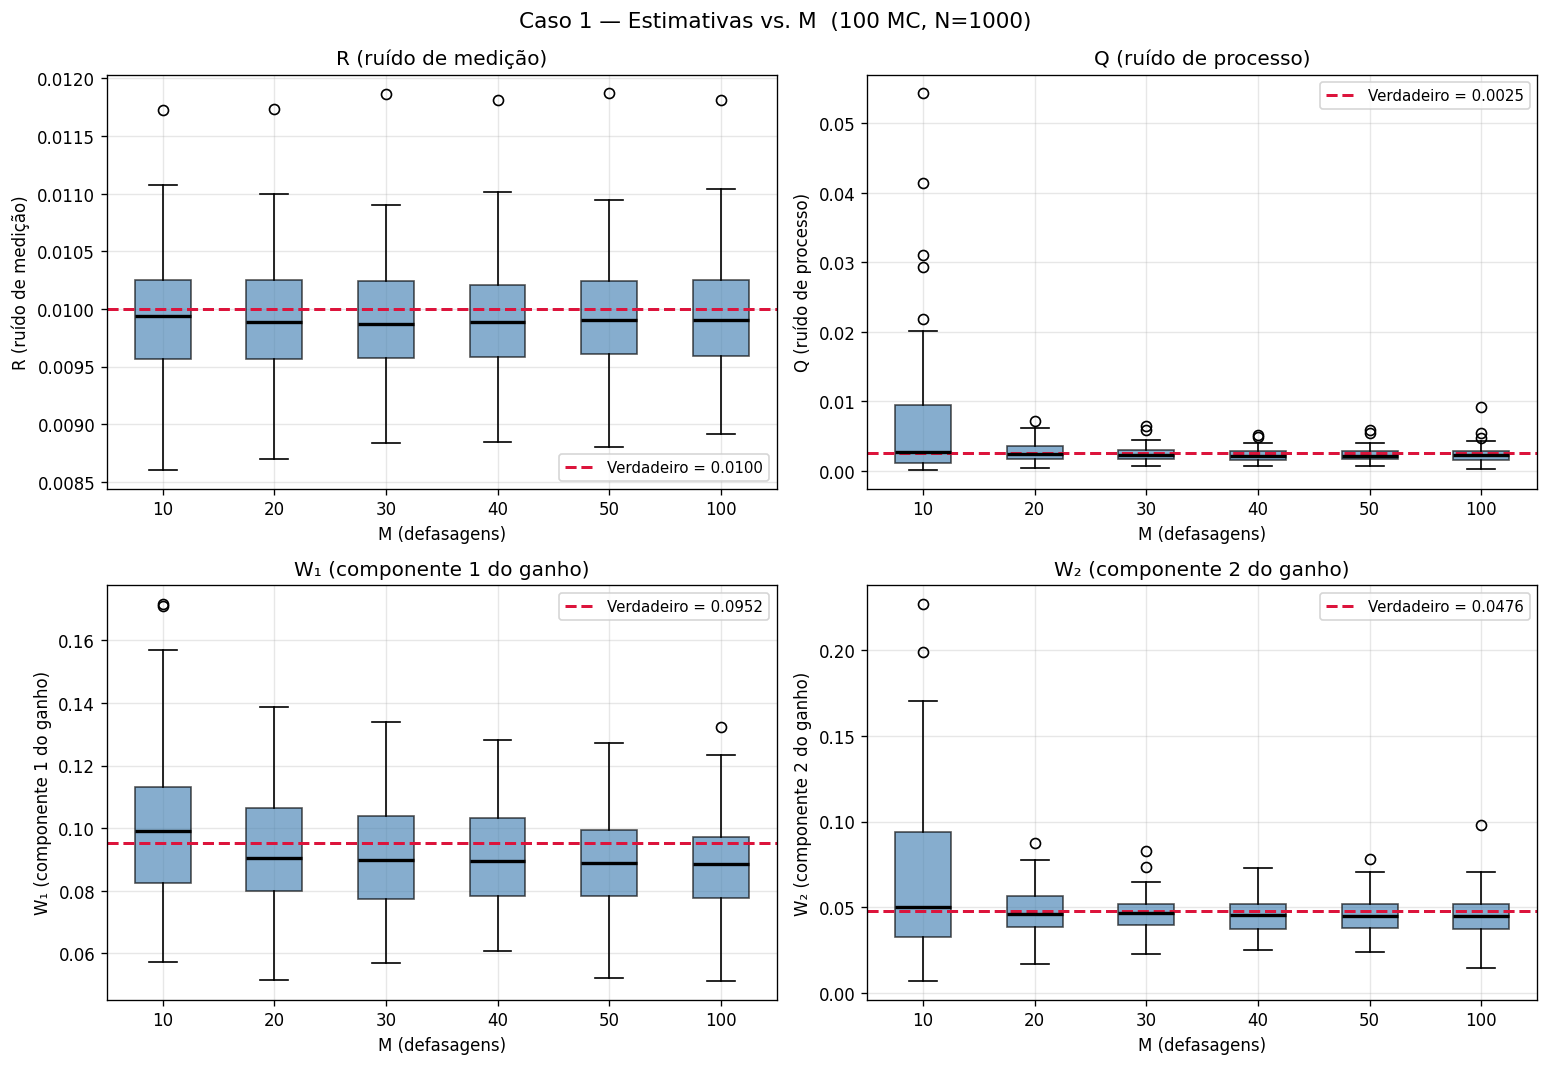
\includegraphics[width=\linewidth]{case1_boxplots.png}
                \caption{Distribuição de $\hat{Q}$ e $\hat{R}$ para cada valor de $M$.
                         Linha tracejada: valor verdadeiro.}
            \end{figure}
        \end{column}
        \begin{column}{0.35\textwidth}
            \vspace{0.4cm}
            \begin{block}{Resultados ($M = 40$)}
                \begin{tabular}{lcc}
                    \toprule
                    & $\hat{R}$ & $\hat{Q}$ \\
                    \midrule
                    Verdadeiro & 0,010 & 0,0025 \\
                    Média      & 0,00993 & 0,00229 \\
                    IC 2,5\%   & 0,00909 & 0,00084 \\
                    IC 97,5\%  & 0,01091 & 0,00391 \\
                    \bottomrule
                \end{tabular}
            \end{block}
            \vspace{0.2cm}
            Valor verdadeiro \textbf{dentro} do IC 95\%
            em todas as realizações $\checkmark$
        \end{column}
    \end{columns}
\end{frame}

% ---------------------------------------------------------------------------
\begin{frame}{NIS --- O Que é e Como Usar}
    \begin{block}{NIS --- Normalized Innovation Squared (eq. 191)}
        \[
            \varepsilon(k) = \boldsymbol{\nu}(k)'\,S^{-1}\,\boldsymbol{\nu}(k)
        \]
        Mede o quanto a inovação é ``surpreendente'' dado o tamanho esperado
        da covariância da inovação $S$.
    \end{block}
    \vspace{0.2cm}
    \begin{columns}[T]
        \begin{column}{0.52\textwidth}
            \textbf{Propriedade teórica:}
            Para um filtro \textbf{bem calibrado} (com os $Q$ e $R$ corretos):
            \[
                \varepsilon(k) \sim \chi^2(n_z), \qquad
                \mathbb{E}[\varepsilon(k)] = n_z
            \]
            Plotamos $\varepsilon(k)/n_z$ --- valor esperado igual a 1.
        \end{column}
        \begin{column}{0.45\textwidth}
            \begin{alertblock}{Interpretação}
                \begin{itemize}
                    \item NIS $\gg 1$: filtro subestima a incerteza
                          ($Q$ ou $R$ pequenos demais)
                    \item NIS $\ll 1$: filtro superestima a incerteza
                          ($Q$ ou $R$ grandes demais)
                    \item NIS $\approx 1$: filtro \textbf{consistente} $\checkmark$
                \end{itemize}
            \end{alertblock}
        \end{column}
    \end{columns}
\end{frame}

% ---------------------------------------------------------------------------
\begin{frame}{Caso 1 --- Consistência pelo Teste NIS}
    \begin{columns}[T]
        \begin{column}{0.62\textwidth}
            \begin{figure}
                \centering
                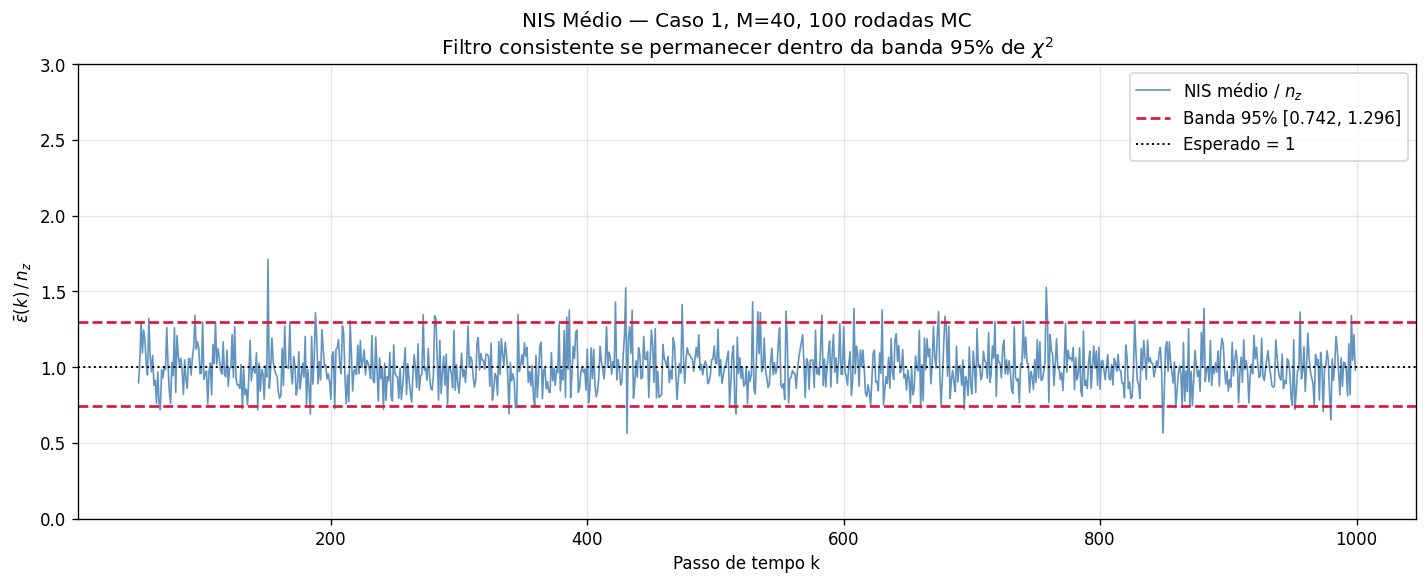
\includegraphics[width=\linewidth]{case1_nis.png}
                \caption{NIS ao longo do tempo para o Caso 1 ($M=40$, média sobre
                         100 realizações). Faixa sombreada: intervalo 95\% da $\chi^2(1)$.}
            \end{figure}
        \end{column}
        \begin{column}{0.35\textwidth}
            \vspace{0.5cm}
            \begin{block}{Diagnóstico}
                \begin{itemize}
                    \item NIS médio $\approx 1{,}0$
                    \item Fração dentro da banda 95\%: alta $\checkmark$
                    \item Sem tendência sistemática
                \end{itemize}
            \end{block}
            \vspace{0.3cm}
            O filtro com as covariâncias estimadas pelo algoritmo de
            6 passos é \textbf{estatisticamente consistente}.
        \end{column}
    \end{columns}
\end{frame}

% ===========================================================================
\section{Aplicação: EKF para Rastreamento de Trajetória}
% ===========================================================================

% ---------------------------------------------------------------------------
\begin{frame}{Aplicação EKF --- Modelo do Sistema}
    \begin{columns}[T]
        \begin{column}{0.50\textwidth}
            \textbf{Modelo PVA (posição-velocidade-aceleração):}
            \[
                \mathbf{x} = [p_x,\;\dot{p}_x,\;\ddot{p}_x,\;
                               p_y,\;\dot{p}_y,\;\ddot{p}_y]^\top \in \mathbb{R}^6
            \]

            \textbf{Medição não linear (distâncias):}
            \[
                z_i(k) = \sqrt{(p_x - a_{xi})^2 + (p_y - a_{yi})^2} + v_i
            \]
            $4$ estações base: $\text{S}_1{=}(0,0)$, $\text{S}_2{=}(600,600)$,
            $\text{S}_3{=}(0,600)$, $\text{S}_4{=}(600,0)$ (metros)
        \end{column}
        \begin{column}{0.47\textwidth}
            \begin{block}{Parâmetros}
                \begin{tabular}{ll}
                    Período $T_s$ & $1{,}0$ s \\
                    $N$ & 100 passos \\
                    $\sigma_R$ & $1{,}0$ m (ruído sensor) \\
                    $S_a$ & $0{,}01$ m²/s³ (Singer) \\
                    $R = \sigma^2 I_4$ & $= I_4$ \\
                \end{tabular}
            \end{block}
            \vspace{0.2cm}
            \begin{alertblock}{Por que EKF?}
                A medição é \textbf{não linear}. O Jacobiano $H_k$
                é recalculado a cada passo na estimativa a priori
                $\hat{\mathbf{x}}(k|k{-}1)$.
            \end{alertblock}
        \end{column}
    \end{columns}
\end{frame}

% ---------------------------------------------------------------------------
\begin{frame}{EKF --- Trajetória Quadrada}
    \begin{columns}[T]
        \begin{column}{0.49\textwidth}
            \begin{figure}
                \centering
                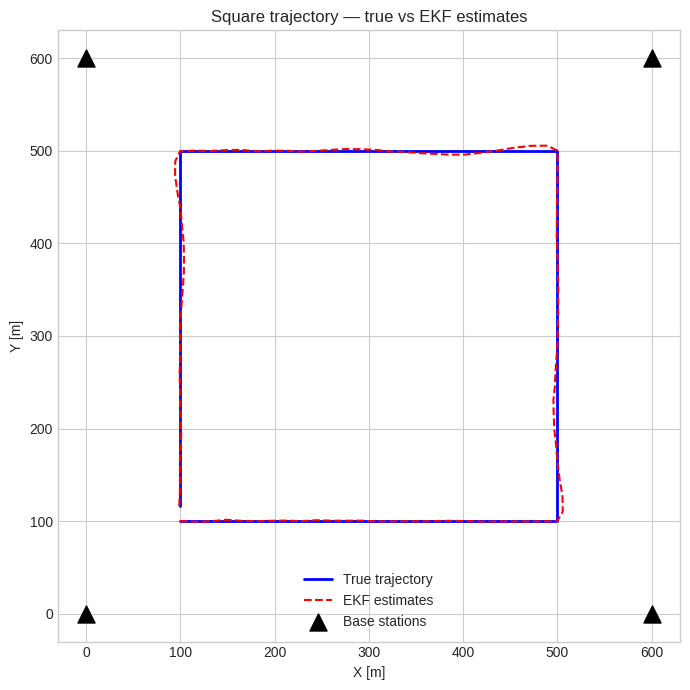
\includegraphics[width=\linewidth]{square_trajectory.png}
                \caption{Trajetória quadrada: percurso real vs.\ estimado pelo EKF.}
            \end{figure}
        \end{column}
        \begin{column}{0.49\textwidth}
            \begin{figure}
                \centering
                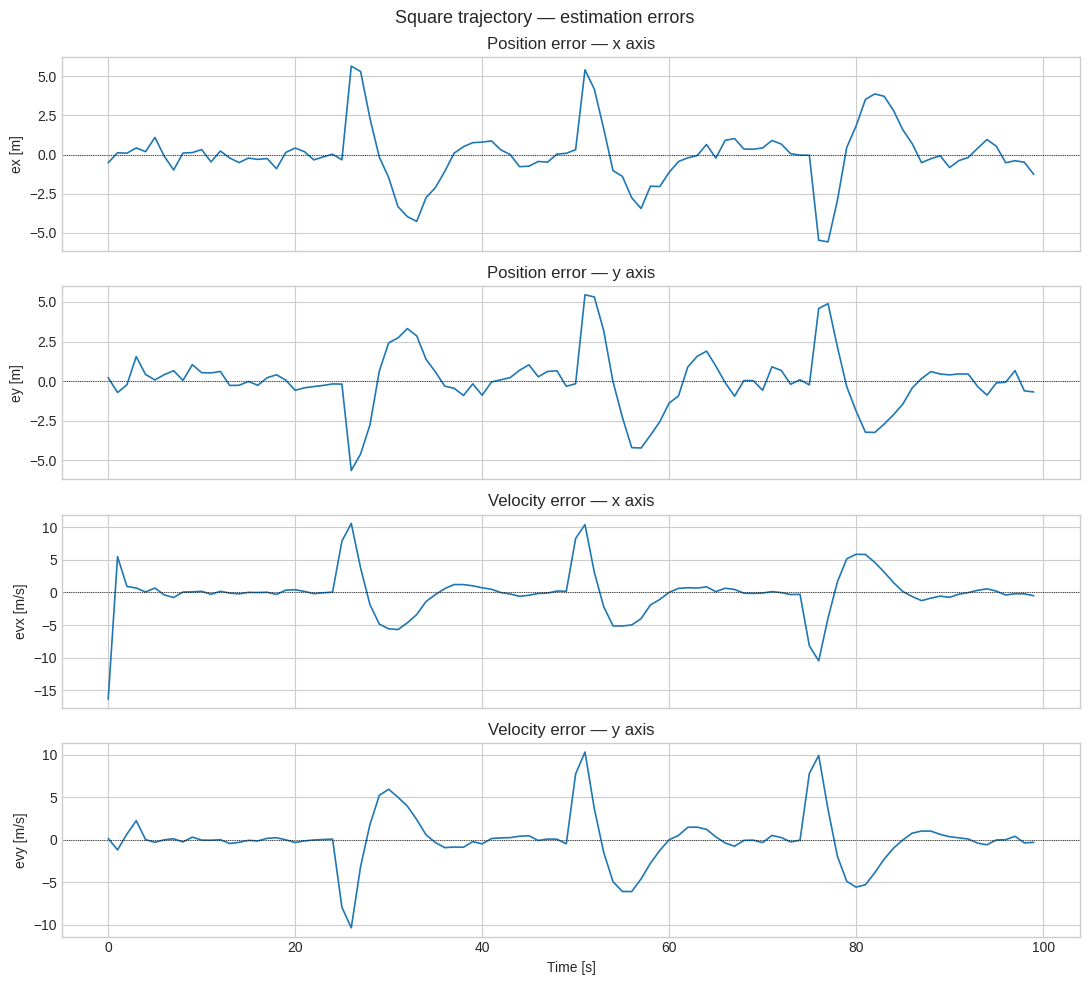
\includegraphics[width=\linewidth]{square_trajectory_errors.png}
                \caption{Erros de posição e velocidade ao longo do tempo.}
            \end{figure}
        \end{column}
    \end{columns}
    \vspace{0.15cm}
    \centering
    \small
    RMSE posição: $\approx 0{,}39$ m \quad|\quad
    RMSE velocidade: $\approx 0{,}31$ m/s \quad|\quad
    Picos nos cantos (mudança abrupta de aceleração)
\end{frame}

% ---------------------------------------------------------------------------
\begin{frame}{EKF --- Trajetória Circular}
    \begin{columns}[T]
        \begin{column}{0.49\textwidth}
            \begin{figure}
                \centering
                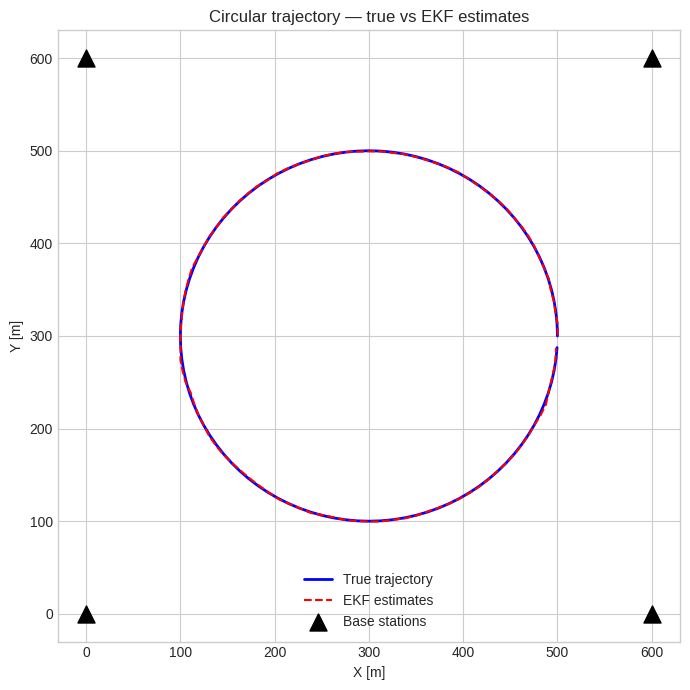
\includegraphics[width=\linewidth]{circular_trajectory.png}
                \caption{Trajetória circular: percurso real vs.\ estimado pelo EKF.}
            \end{figure}
        \end{column}
        \begin{column}{0.49\textwidth}
            \begin{figure}
                \centering
                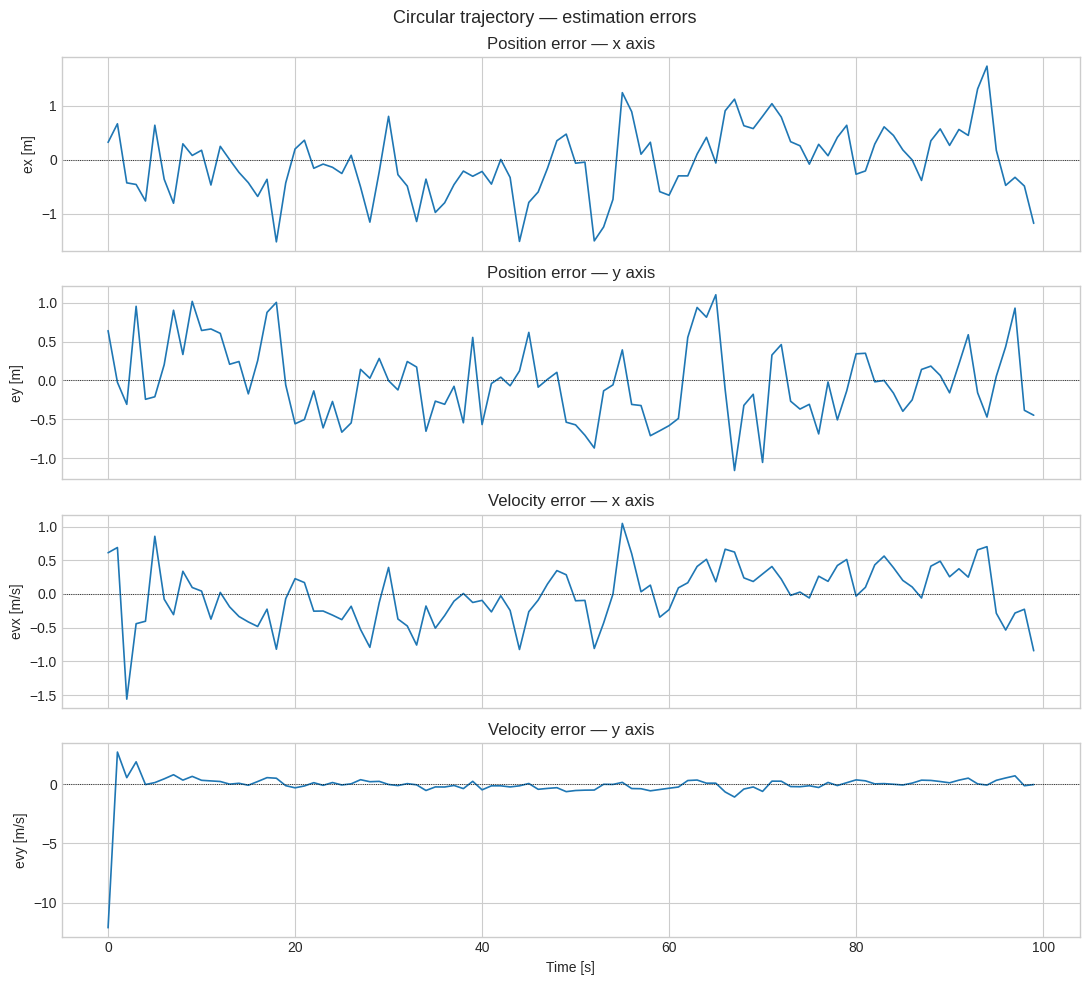
\includegraphics[width=\linewidth]{circular_trajectory_errors.png}
                \caption{Erros de posição e velocidade ao longo do tempo.}
            \end{figure}
        \end{column}
    \end{columns}
    \vspace{0.15cm}
    \centering
    \small
    RMSE posição: $\approx 0{,}42$ m \quad|\quad
    RMSE velocidade: $\approx 0{,}35$ m/s \quad|\quad
    Movimento suave; erros mais uniformes que na trajetória quadrada
\end{frame}

% ---------------------------------------------------------------------------
\begin{frame}{EKF --- Validação pelo Teste NIS}
    \begin{columns}[T]
        \begin{column}{0.60\textwidth}
            \begin{figure}
                \centering
                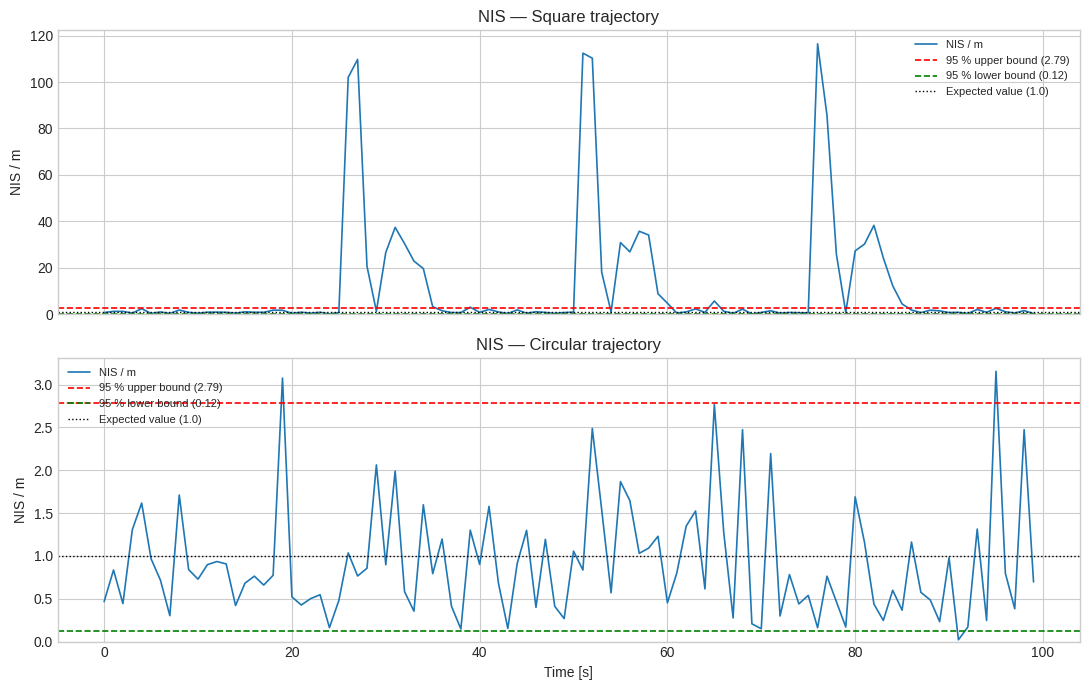
\includegraphics[width=\linewidth]{ekf_nis.png}
                \caption{NIS normalizado para as duas trajetórias.
                         Linhas tracejadas: limites 95\% da $\chi^2(4)/4$.}
            \end{figure}
        \end{column}
        \begin{column}{0.37\textwidth}
            \vspace{0.3cm}
            \begin{block}{Resultados NIS}
                \small
                \begin{tabular}{lc}
                    \toprule
                    Trajetória & Dentro da banda 95\% \\
                    \midrule
                    Quadrada   & 75\% \\
                    Circular   & 84\% \\
                    \bottomrule
                \end{tabular}
            \end{block}
            \vspace{0.3cm}
            \textbf{Interpretação:} desempenho aceitável,
            considerando a linearização aproximada do EKF
            e o descasamento do modelo nos cantos da trajetória
            quadrada.
        \end{column}
    \end{columns}
\end{frame}

% ===========================================================================
\section{Conclusões}
% ===========================================================================

% ---------------------------------------------------------------------------
\begin{frame}{Conclusões}
    \begin{block}{Algoritmo de Seis Passos}
        O método de Zhang et al. (2020) estima $Q$ e $R$ com RMSE
        baixo sem qualquer conhecimento a priori dos valores reais.
        Melhor resultado para $M=40$ ($N=1000$):
        RMSE($\hat{R}$) $= 5{,}1\times10^{-4}$,
        RMSE($\hat{Q}$) $= 9{,}3\times10^{-4}$.
    \end{block}
    \vspace{0.2cm}
    \begin{block}{Sensibilidade ao Parâmetro $M$}
        $M=40$ é o ponto ótimo para este cenário ($N=1000$):
        valores maiores não melhoram significativamente a estimação.
    \end{block}
    \vspace{0.2cm}
    \begin{block}{Aplicação com EKF}
        Rastreamento 2D com medições de distância não lineares:
        RMSE de posição $\approx 0{,}4$ m, NIS dentro da faixa 75--84\%
        (ligeiro descasamento esperado pela linearização do EKF).
    \end{block}
    \vspace{0.2cm}
    \centering
    \small
    \textbf{Referência:} Zhang et al. (2020), \textit{IEEE Access}, vol. 8,
    pp.\ 59362--59388. DOI: 10.1109/ACCESS.2020.2982407
\end{frame}

% ---------------------------------------------------------------------------
% Slide final
% ---------------------------------------------------------------------------
\begin{frame}
    \vfill
    \begin{center}
        {\Huge \textbf{Obrigado!}}\\[1.5cm]
        {\large Mateus Pincho de Oliveira}\\[0.3cm]
        {\normalsize Universidade Federal de Campina Grande -- UFCG}\\[0.3cm]
        {\normalsize Sistemas Inteligentes -- 2026}
    \end{center}
    \vfill
\end{frame}

\end{document}
